% Zero-Copy CSI Streaming for Open-Source SDR Wi-Fi Sensing
% ComEX (IEICE Communications Express) layout draft
% Compile: xelatex paper.tex
\documentclass[10pt,a4paper]{article}
\usepackage[utf8]{inputenc}
\usepackage[T1]{fontenc}
\usepackage{lmodern}
\usepackage[a4paper,margin=2.1cm,top=2.2cm]{geometry}
\usepackage{graphicx}
\usepackage{booktabs}
\usepackage{array}
\usepackage{caption}
\usepackage[colorlinks=true,linkcolor=black,urlcolor=blue]{hyperref}
\captionsetup{font=small,labelfont=bf}
\setlength{\parskip}{2pt}

\begin{document}

\begin{center}
  {\LARGE\bfseries Zero-Copy CSI Streaming for Open-Source SDR Wi-Fi Sensing}\\[6pt]
  [Author A], [Author B], and [Author C]\\[2pt]
  {\small [Affiliation, City, Country]}
\end{center}

\vspace{2mm}
\noindent\textbf{Abstract}\hspace{0.5em}---\hspace{0.5em}
Channel State Information (CSI) is the raw material for device-free Wi-Fi
sensing, whose fidelity scales with the delivered CSI frame rate. We quantify
and remove the delivery bottleneck of the stock CSI path of Openwifi, an
open-source IEEE 802.11 SDR, on a self-ported Zynq-7020/AD9361 board. The
stock path polls each frame through the kernel netlink layer and copies it
twice before reaching userspace. We redesign it as a zero-copy path in which
the FPGA streams frames through a continuous AXI DMA into a coherent ring
buffer exposed via mmap and poll. Across a 1--20\,Mbit/s fixed-rate uplink
sweep, the redesign lowers capture CPU by up to $\times$3.9, keeps per-frame
cost linear in delivered frames, and tracks the full stream where the stock
path drops capture. A TSF-monotonicity and equalizer-amplitude cross-check
confirms no dirty reads.

\medskip
\noindent\textbf{Keywords:} openwifi, IEEE 802.11, channel state information,
zero-copy streaming, software-defined radio, Wi-Fi sensing

\vspace{2mm}
\hrule
\vspace{3mm}

\section{Introduction}

CSI is the raw material for device-free wireless sensing --- activity
recognition, presence detection, passive localization --- and sensing accuracy
hinges on CSI \emph{frame rate}: snapshots must be captured fast enough to
resolve human-scale dynamics, pushing the per-frame processing rate to the
kilo-hertz range and beyond.

Openwifi is the leading open-source Wi-Fi transceiver for this kind of
research: it runs a fully open MAC/PHY on an FPGA+SDR (AD9361) and exposes CSI
through a community ``side channel'' \cite{openwifi}. Yet its stock CSI path
was designed for debugging, not sustained sensing: the driver polls each frame
through the kernel netlink layer on a fixed 1\,ms tick and pushes it over UDP,
crossing the kernel/userspace boundary twice and copying out of a per-transfer
DMA buffer. What that design \emph{costs}, however, has never been quantified:
we provide the first measurement.

This letter makes three contributions for open-source SDR Wi-Fi sensing, using
openwifi on a self-ported RK-ZYNQ7020-F board as the vehicle:
\begin{enumerate}
  \item the \textbf{first quantitative characterization of the stock openwifi
        CSI delivery cost}: under an identical $\sim$1.1\,kframes/s uplink,
        the stock netlink$\rightarrow$UDP path spends $\sim$\textbf{15.2\%}
        of a core in the capture process alone; we decompose where those
        cycles go (polling quantization, per-transfer DMA map/unmap, two CPU
        copies);
  \item a \textbf{zero-copy re-design} of that path --- a continuous DMA
        front-end streaming frames into a \emph{coherent ring buffer} with a
        single mapping (no per-transfer map/unmap, no CPU copy), exposed via
        \textbf{mmap + poll} --- measured across a 1--20\,Mbit/s fixed-rate
        sweep with a consistent end-to-end (UDP-exit) methodology: up to
        $\sim$\textbf{3.9$\times$} lower capture CPU, linear per-frame cost,
        and \textbf{no dirty reads} against the baseline;
  \item a \textbf{reproducible benchmark methodology} (fixed-rate uplink,
        mutually exclusive drivers, multi-round mean$\pm$std protocol) so the
        numbers can be re-obtained and extended on any openwifi-compatible
        board.
\end{enumerate}

Zero-copy delivery itself is a mature pattern (DPDK, AF\_XDP, io\_uring, V4L2
\cite{dpdk,afxdp,iouring}); the contribution is what it buys on an open Wi-Fi
SDR --- a quantified account of the stock path's cost, a redesign that
removes it, and a reproducible methodology. The freed CPU headroom is exactly
what a sensing algorithm needs on the same embedded processor.

\section{Bottleneck Analysis of the Stock CSI Path}

To motivate the design we first characterise the baseline \texttt{side\_ch}
path.

\textbf{Path.} openwifi's CSI is produced in the FPGA (\texttt{side\_ch.v})
and delivered on demand. \texttt{side\_ch\_ctl} polls over netlink; each
request triggers an AXI DMA of one frame into a kernel \texttt{kmalloc}
buffer, which is then copied into a netlink message and forwarded to a
userspace UDP daemon:
\begin{center}
  \texttt{FPGA(side\_ch.v) $\rightarrow$ kernel buf $\rightarrow$ netlink msg
  $\rightarrow$ UDP $\rightarrow$ userspace}
\end{center}
Fig.~\ref{fig:arch} contrasts this stock path with the proposed zero-copy
design.

\begin{figure}[t]
  \centering
  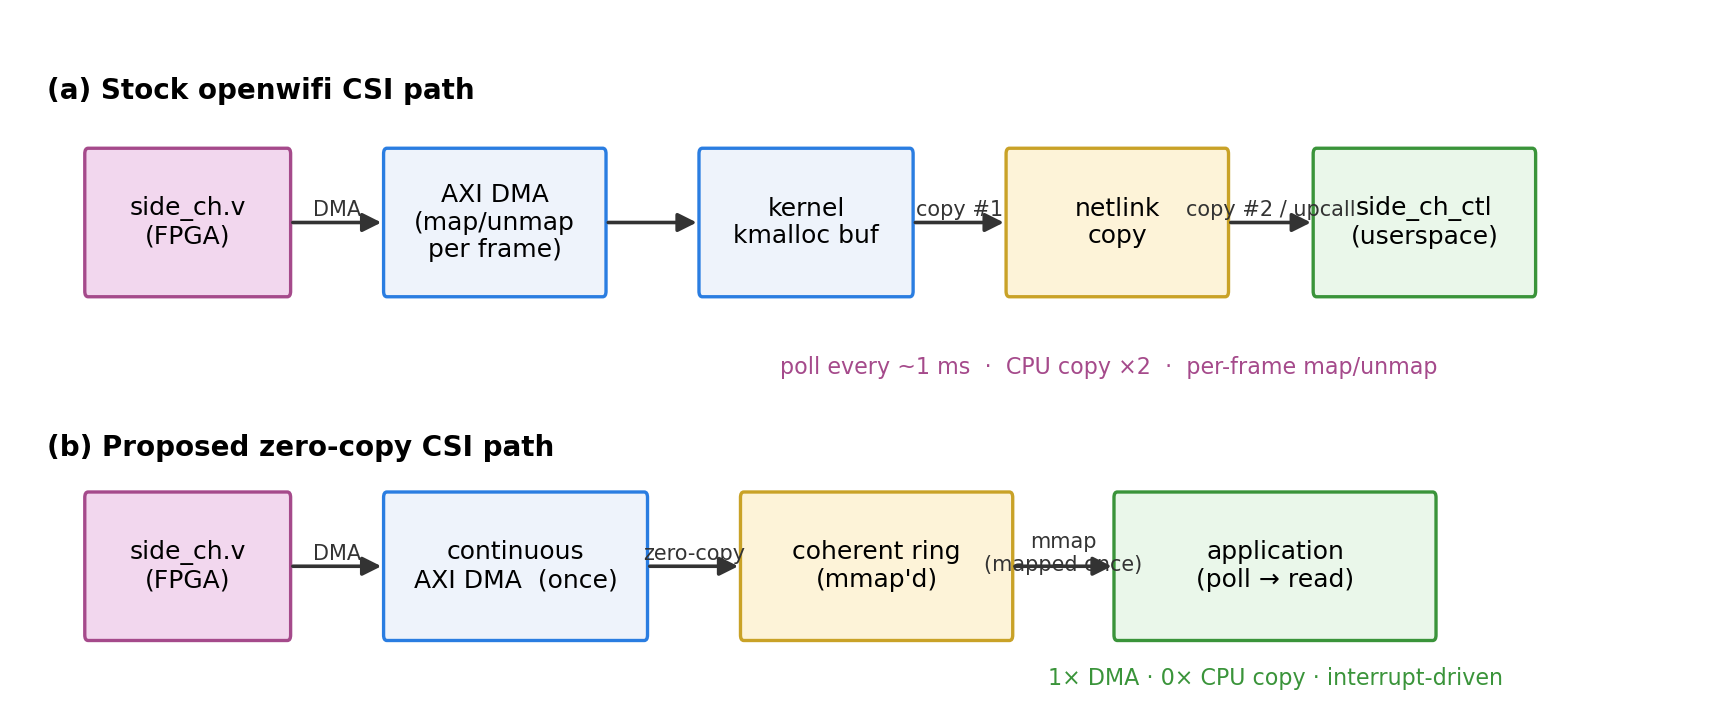
\includegraphics[width=0.92\linewidth]{figures/fig1_architecture.png}
  \caption{System architecture. (a) Stock openwifi path:
  \texttt{side\_ch.v $\rightarrow$ AXI DMA (map/unmap per frame) $\rightarrow$
  kmalloc $\rightarrow$ netlink copy $\rightarrow$ side\_ch\_ctl $\rightarrow$
  UDP recv}, annotating ``2$\times$CPU copy'', ``1\,ms poll''. (b) Proposed
  path: \texttt{side\_ch.v $\rightarrow$ continuous AXI DMA $\rightarrow$
  coherent ring $\rightarrow$ mmap $\rightarrow$ poll $\rightarrow$
  application}, annotating ``1$\times$DMA, 0$\times$CPU copy'',
  ``interrupt-driven''.}
  \label{fig:arch}
\end{figure}

\textbf{Four costs stand out} for a sensing workload:
\begin{enumerate}
  \item \textbf{Polling quantization.} The 1\,ms poll tick bounds how early a
        frame is delivered and injects quantization jitter into the observed
        timestamps (Section~4, Fig.~\ref{fig:sweep}).
  \item \textbf{Per-transfer DMA map/unmap.} Every poll maps, fills, unmaps a
        buffer --- page-attribute flushes that cost cycles and interact
        poorly with throughput.
  \item \textbf{Two CPU copies.} DMA $\rightarrow$ netlink copy, plus the
        protocol-stack copy toward the UDP socket --- the frames are moved
        twice through the CPU cache.
  \item \textbf{Copy work lands on the same core} that a sensing classifier
        would use: \texttt{side\_ch\_ctl} alone used $\sim$5.7\% of one core
        at 1\,Mbit/s and $\sim$17.7\% at 20\,Mbit/s (Section~4, Table~1).
\end{enumerate}

The conclusion: the bottleneck is not bandwidth (a CSI frame is
$\sim$0.5--1\,KB) but per-frame CPU work and timing slop, so a sensing
pipeline benefits more from removing copy/poll overhead than from adding DMA
width --- pointing directly at a zero-copy, interrupt-driven ring design.

\section{System Design: Zero-Copy Ring Streaming}

Our design keeps the same Silicon (Zynq-7020, AXI DMA, AD9361) but changes the
data path so a CSI frame is DMA'd \textbf{once} into a shared, coherent buffer
the consumer already has mapped.

\textbf{Continuous DMA to a coherent ring.} The driver allocates one
\texttt{dma\_alloc\_coherent} buffer and programs the AXI DMA
(\texttt{rx\_dma\_s2mm}) to write each completed frame into the next ring
slot, keeping the buffer permanently mapped (no map/unmap per frame):
\begin{center}
  \texttt{FPGA(side\_ch.v) $\rightarrow$ coherent ring buffer $\rightarrow$
  mmap $\rightarrow$ userspace}
\end{center}
Because the buffer is DMA-coherent (uncached on Zynq) the producer index is
visible to userspace immediately after each transfer, with no round-trip into
the kernel.

\textbf{Ring layout} (Fig.~\ref{fig:ring}): the first page holds a metadata
header (\texttt{producer\_idx}, \texttt{frame\_seq}, \texttt{slot\_size},
\texttt{num\_eq}, \dots); the rest holds $N$ fixed-size slots, one CSI frame
each (default \texttt{num\_eq=8}, $16\times4$\,KB). The frame layout keeps the
openwifi convention --- symbol 0 is the 64-bit 802.11 TSF timestamp ($\mu$s),
symbol 1 the phase offset, then 56 complex subcarriers and \texttt{num\_eq}
equalizer blocks --- so existing PHY consumers are unchanged.

\begin{figure}[t]
  \centering
  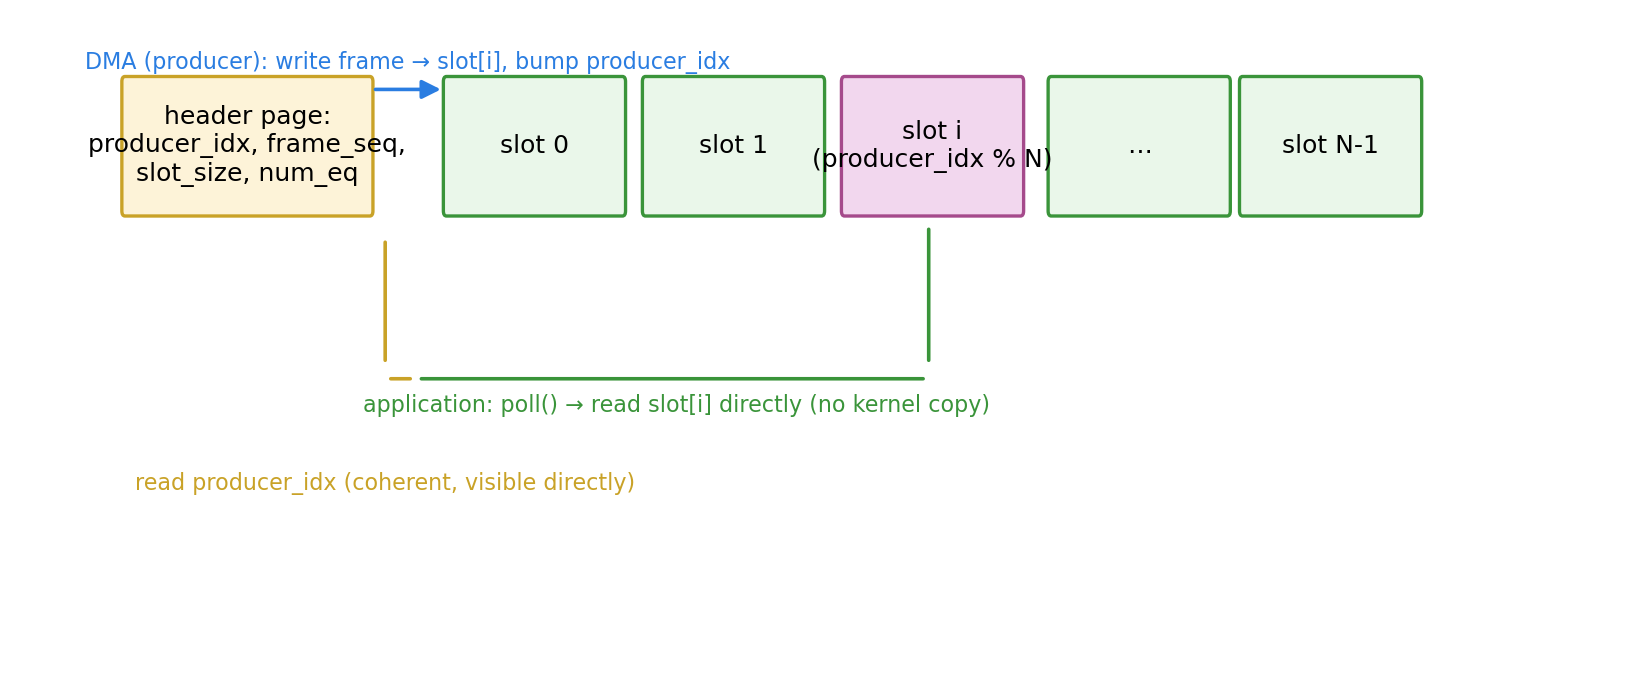
\includegraphics[width=0.88\linewidth]{figures/fig2_ring.png}
  \caption{Coherent ring buffer data-flow: metadata header page + $N$ slots;
  ``DMA (producer) writes slot[$i$]'', ``poll'' notifies, ``app reads
  slot[$i$]''; the \texttt{producer\_idx} advances and is read directly by
  userspace.}
  \label{fig:ring}
\end{figure}

\textbf{mmap + poll.} Userspace \texttt{mmap}s the ring
(\texttt{MAP\_SHARED}, read-only) and \texttt{poll()}s the device; on a
DMA-completion interrupt the driver bumps \texttt{producer\_idx} and wakes
the poller. The consumer reads the new slots directly --- no kernel copy, no
poll quantization, no syscall per frame.

\textbf{Control surface} (ioctls): \texttt{START/STOP}, \texttt{SET\_NUM\_EQ},
\texttt{GET\_STATS} (\texttt{dma\_err\_count}, \texttt{frame\_seq}). The
driver loads with \texttt{auto\_start=0} and does not stream until START, so
installing it does not disturb beaconing.

\section{Evaluation}

\textbf{Setup (fixed, reproducible).} Board RK-ZYNQ7020-F (Zynq-7020, 32-bit,
no SMMU), AD9361, 2.4\,GHz AP (channel 6, +37\,kHz CFO), an X230 client
(Wi-Fi power save off) generating a fixed-rate UDP uplink (iperf3
$\rightarrow$ 5201). Both paths are measured identically \textbf{end to end}
--- every frame is forwarded over UDP to a loopback receiver
(192.168.10.1:4000) --- so the only difference is the eliminated
driver$\rightarrow$user-space copy. Each point aggregates $3\times60$\,s
rounds per path (mean$\pm$std, \texttt{num\_eq=8}); stalled rounds
($<$50\% of group median) were re-run, not averaged.

\begin{table}[t]
  \centering
  \caption{Fixed-rate uplink sweep (mean$\pm$std, 3 rounds $\times$ 60\,s).}
  \label{tab:sweep}
  \begin{tabular}{lcccc}
    \toprule
    uplink & baseline fps & baseline CPU\% & mmap fps & mmap CPU\% \\
    \midrule
    1 Mbit/s  & $104.6\pm2.5$   & $5.74\pm0.04$ & $111.6\pm5.1$    & $1.49\pm0.08$ \\
    5 Mbit/s  & $474.6\pm9.2$   & $8.56\pm0.09$ & $516.2\pm4.2$    & $6.13\pm0.02$ \\
    10 Mbit/s & $853.5\pm94.1$  & $11.06\pm0.73$ & $836.6\pm168.3$ & $9.60\pm1.93$ \\
    20 Mbit/s & $1788.7\pm9.5$  & $17.69\pm0.13$ & $2084.3\pm30.2$ & $23.58\pm0.52$ \\
    \bottomrule
  \end{tabular}
\end{table}
(Explicit loss is 0.00\% and DMA errors 0 at every point, both paths.)

Three observations. \textbf{(i) At 1--10\,Mbit/s} the zero-copy path delivers
equal-or-more frames with strictly less capture CPU --- \textbf{3.9$\times$
less at 1\,Mbit/s}, where the stock path's fixed 1\,ms poll + netlink
overhead dominates, narrowing to $\times$1.15 at 10\,Mbit/s. \textbf{(ii) At
20\,Mbit/s} the stock path starts dropping capture: it delivers only
1789\,fps vs 2084\,fps for mmap ($-$14\%), because its one-shot per-poll DMA
and netlink copy cannot keep up with the sustained stream, while the mmap
path tracks the full offered load. Per delivered frame the mmap cost is
nearly flat (0.011--0.013\,\%/fps across the whole sweep --- a purely
per-frame, linear cost), whereas the baseline's fixed polling overhead makes
it $\sim$4$\times$ more expensive per frame at 1\,Mbit/s. \textbf{(iii) No
frames are lost} on either path; the stock shortfall appears as
\emph{un-captured} CSI frames --- precisely the frames a sensing application
needs.

\textbf{Data consistency (no dirty reads).} Removing the CPU copy must not
trade speed for corruption. We compared the two raw streams on the same
channel (500-frame window, \texttt{num\_eq=8}): the 64-bit 802.11 TSF is
strictly monotonic in the baseline (0/499 violations); the mmap stream shows
8 regressions --- complete-duplicate slots or beacon-aligned FPGA
re-emissions, \textbf{0 torn frames} ($\sim$1.37\% over the full 31,387-frame
capture). The equalizer amplitude profile is near-identical between paths
(mean-vector correlation 1.0000, per-frame 0.9975). Verdict:
\textbf{PASS --- no dirty reads}.

\begin{figure}[t]
  \centering
  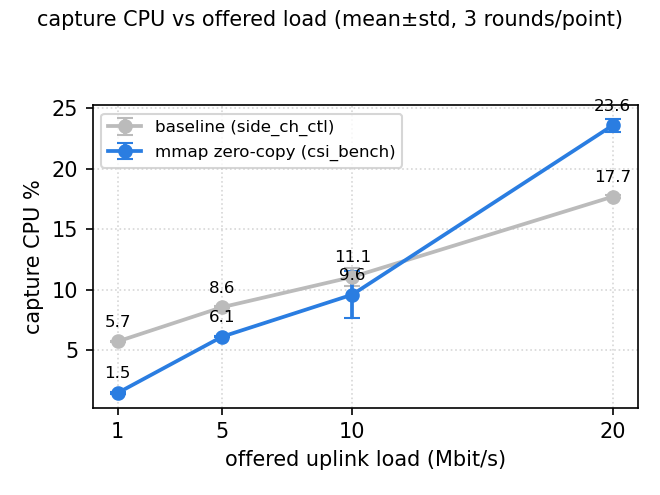
\includegraphics[width=0.92\linewidth]{figures/sweep_cpu_vs_rate.png}
  \caption{(a) Capture CPU vs uplink rate (Table~\ref{tab:sweep}, both
  curves): the mmap curve is flat per frame while the baseline carries a
  fixed polling tax and ends 14\% short of the stream at 20\,Mbit/s; (b) CDF
  of inter-frame TSF interval: p50 341\,$\mu$s on both paths at
  5--20\,Mbit/s, p95 554--620\,$\mu$s (baseline) vs 567--600\,$\mu$s (mmap).}
  \label{fig:sweep}
\end{figure}

\textbf{Claim.} The zero-copy path's capture CPU is linear in delivered
frames ($\approx$0.011\,\%/fps) and lower wherever the stock path keeps pace;
the data-consistency check confirms these gains come with no dirty reads.

\section{Conclusion}

We showed that the CSI capture path of an open Wi-Fi SDR can be redrawn as a
zero-copy, interrupt-driven ring whose capture cost is linear in the
delivered frame rate and lower than the stock path wherever the stock path
keeps pace --- and that at high offered rates the stock path begins dropping
capture while the ring tracks the full stream --- all with no dirty reads,
verified on a self-ported board with a reproducible methodology. The released
compute is the headroom wireless-sensing algorithms on the embedded processor
need. Future work ties this ring to deterministic (TSN-like) delivery and
closes the loop with on-board learnable sensing.

\begin{thebibliography}{9}
\bibitem{openwifi} X.~Jiao, W.~Liu, M.~Mehari, M.~Aslam, and I.~Moerman,
``openwifi: A free and open-source IEEE 802.11 SDR implementation on SoC,''
in \emph{Proc. IEEE 91st Vehicular Technology Conference (VTC2020-Spring)},
Antwerp, Belgium, May 2020.
\bibitem{ad9361} Analog Devices, ``AD9361: RF Agile Transceiver,'' Datasheet,
2017.
\bibitem{csisurvey} Y.~Ma, G.~Zhou, and S.~Wang, ``WiFi sensing with channel
state information: A survey,'' \emph{ACM Computing Surveys}, vol.~52, no.~3,
Art.~no.~46, Jun. 2019.
\bibitem{dpdk} Intel, ``Data Plane Development Kit (DPDK),'' [Online].
Available: \url{https://dpdk.org}
\bibitem{afxdp} K.~Karlsson and M.~T\"orp, ``The path to DPDK speeds for
AF\_XDP,'' \emph{Linux Plumbers Conference}, Vancouver, Canada, Nov. 2018.
\bibitem{iouring} J.~Axboe, ``Efficient IO with io\_uring,'' \emph{Linux
Plumbers Conference}, Lisbon, Portugal, Sep. 2019.
\end{thebibliography}

\end{document}
